\section{TO DEFINE}
\label{context}

\subsection{Les planificateurs d'E/S}

Dans leur fonctionnement, les ordonnanceurs de lecture (sortie) et d'écriture 
(entrée) tentent d'améliorer le débit en réorganisant l'accès aux requêtes dans 
un ordre linéaire basé sur les adresses logiques des données sur le disque, en 
essayant de les fusionner. Bien que cela puisse augmenter le débit global, 
certaines requêtes d'E/S peuvent attendre trop longtemps, provoquant des 
problèmes de latence et des fois de famine. Les planificateurs d'E/S tentent 
d'équilibrer le besoin d'un débit élevé tout en essayant de partager 
équitablement les requêtes d'E/S entre les processus.

Différentes approches ont été adoptées pour divers planificateurs d'E/S et 
chacun a ses propres forces et faiblesses et de manière générale, il n'y a pas 
de planificateur d'E/S par défaut parfait pour toute la gamme de requêtes d'E/S 
qu'un système peut rencontrer. 

\subsection{État de l'art}

Historiquement, les premiers algorithmes d'ordonnancement qui ont été 
développés se sont basés sur la structure interne des disques durs de l'époque, 
que l'on retrouve aujourd'hui encore dans beaucoup d'ordinateur. Cette 
structure organisée par secteurs de données sur plateaux était lue par une tête 
de lecture unique, limitant ainsi les actions possibles sur le disque à une 
seule écriture ou une seule lecture à la fois. Les algorithmes de l'époque ont 
donc été développés en conséquence, et sont devenus au fur et à mesure du 
temps obsolètes. La sortie de nouvelles technologies à la mémoire flash, comme 
les disques SSD (Solid-State Drive) ont offert la possibilité de pouvoir 
effectuer plusieurs lectures et plusieurs écritures de manière simultanée. Ces 
nouvelles technologies ont donc donné naissance à de nouveaux algorithmes, 
comme BFQ en 2003, ou Kyber, développé en 2017 par Facebook.

Aujourd'hui dans Linux il existe plusieurs ordonnanceurs, tous ayant une 
utilité situationnelle et de manière générale, ils se distinguent entre deux 
catégories. Première-ment il y a les ordonnanceurs à file d'attente simple, ce 
sont les premiers qui ont existé et qui sont maintenant dépréciés dans les 
versions de Linux actuelles (depuis la version 5.3). Puis il y a les 
ordonnanceurs à file d'attente multiples, leur tâche est de distribuer les 
requêtes d'E/S aux différents fils d'exécution du noyau qui seront ensuite 
distribués aux différents processeurs. On retrouvera une liste exhaustive des 
planificateurs existant dans Linux en annexe dans la Table~\ref{tab:politics}.

Tous ces ordonnanceurs ont cependant tous un point commun, ils sont écrits à la 
main par un développeur du noyau Linux. Le projet VeriAMOS essaye de changer 
cet aspect en proposant au développeur n'ayant pas toute la connaissance du 
noyau linux de pouvoir créer son propre planificateur facilement grâce à 
PhaistOS. 

\subsection{Arborescence du projet}

PhaistOS est un DSL comme nous l'avons compris, il a été développé par Nick 
Papoulias (ancien membre de l'équipe Erods) comme sujet de post doctorat. Il 
s'est attelé au développement de PhaistOS avec le langage de programmation 
Ocaml et a organisé l'architecture du projet d'une certaine manière, que l'on 
retrouve dans la Figure~\ref{fig:arch} en annexe.

Dans cette arborescence, on retrouve deux sections principales, et des sections 
secondaires. Concernant les sections principales, on retrouve évidemment le 
DSL, qui contiendra tout l'outillage nécessaire pour couvrir les objectifs de 
VeriAMOS, et on retrouvera aussi ``Matryoshka'', qui permettra au prochain 
developpeur de mettre en place son environement de travail pour effectuer ses 
tests assez facilement. Les sections secondaires comprennent les tests de 
performances ainsi que la documentation générale, mais aussi d'autres moins 
significatives, qui n'ont pas été couvertes par mon stage (comme par exemple 
les fichiers de configuration Gitlab, ou les images Docker qu'avait mis en 
place Nick à l'époque).

\subsection{Fonctionnement du DSL}

Pour que PhaistOS puisse produire un code C à partir d'une politique, il 
faut d'abord que celui-ci puisse lire cette politique et l'interpréter. Avant 
de présenter ce mécanisme, présentons le langage dédié. Pour l'illustrer et 
mieux le comprendre dans la partie qui va suivre, nous nous baserons sur 
l'exemple type de l'ordonnanceur MQ-Deadline (description de l'ordonnanceur en annexe, Table~\ref{tab:politics}).

\subsubsection{Le langage de PhaistOS}
\label{phlang}

La politique utilisateur est écrite avec le langage du DSL PhaistOS et 
permettra de scripter le fonctionnement du planificateur d'E/S. Elle est 
inspirée des précédents DSLs Bossa~\cite{Barreto-Muller:asf2002} et 
Ipanema~\cite{lepers2020provable}, desquels elle soutire une conception basée 
sur des événements. Le DSL PhaistOS définit donc 7 événements, listés dans la 
Table~\ref{tab:phaistos-events}. En plus de devoir définir chacun de ces 
événements, le développeur doit aussi spécifier l'état de l'ordonnanceur (voir 
un exemple avec la politique deadline personnalisée, Figure~\ref
{fig:deadline_state}) et certaines fonctions personnelles si nécessaire. 

\begin{table}[h!t]
    \centering
    \begin{tabular}{|l|l|} \hline
      \textbf{Événement} & \textbf{Description} \\ \hline
      \texttt{INIT} & Initialisation de l'ordonnanceur \\
      \texttt{EXIT} & Nettoyage à la suppression de l'ordonnanceur \\
      \texttt{INSERT} & Enregistrement d'une nouvelle requête à traiter \\
      \texttt{REMOVE} & Suppression d'une requête en attente \\
      \texttt{DISPATCH} & Retourne la prochaine requête à envoyer pour le 
      disque \\
      \texttt{MERGE} & Procède à la fusion de deux requêtes \\
      \texttt{HAS\_WORK} & Indique s'il existe des requêtes en attente \\ \hline
    \end{tabular}
    \caption{List des événements PhaistOS}
    \label{tab:phaistos-events}
\end{table}


\begin{figure}[h!t]
    \centering
    \begin{tabular}{c}
        \begin{lstlisting}[language=Phaistos, linewidth=6cm]
int read_expire = HZ / 2; (*\label{read}*)
int write_expire = 5 * HZ; 
int writes_starved = 2;
int fifo_batch = 16; (*\label{fifo_batch}*)

POLICY { (*\label{policy}*)
    list fifo_list[2]; (*\label{list}*)
    int fifo_expire[2];
    int fifo_batch;
    int writes_starved;
    int batching;
    int starved;
}(*\label{end-policy}*)
        \end{lstlisting}
    \end{tabular}
    \caption{État de la politique Deadline implementé dans PhaistOS}
    \label{fig:deadline_state}
\end{figure}

Dans la Figure~\ref{fig:deadline_state}, les Lignes~\ref{read}~à~\ref
{fifo_batch} décrivent des constantes spécifiques tandis que l'état interne de 
la politique est décrit par la structure \texttt{POLICY} des Lignes~\ref{policy}
~à~\ref{end-policy}. Grâce à ces variables, le développeur pourra assez 
simplement reproduire le comportement de l'algorithme deadline visé en se 
servant de deux listes (Ligne~\ref{list}), qui sont accompagnées d'une API 
proposant des opérations sémantiques comme \texttt{init}, \texttt{append}, 
\texttt{next\_request} ou encore \texttt{is\_empty}. La partie principale du 
planificateur se trouvera dans d'autres blocs que \texttt{POLICY}, comme par 
exemple le bloc \texttt{EVENTS} qui aura à charge de contenir la définition de 
chacun des événements de la Table~\ref{tab:phaistos-events}, la Figure~\ref
{fig:event-code} en annexe donne un aperçu de comment sont gérés certains 
événements pour la politique deadline. Par exemple l'événement \texttt{INIT}, 
appelé à l'initialisation de l'ordonnanceur, a pout but d'initié l'état interne 
de la politique décrit dans la Figure~\ref{fig:deadline_state}. Durant son 
exécution, l'ordonnanceur recevera des requêtes et fera l'appel à l'événement 
\texttt{INSERT} pour les prendre en compte, et appelera \texttt{DISPATCH} pour 
élir la prochaine à envoyer au disque. \texttt{REMOVE} sera appelé après un 
\texttt{DISPATCH} ou un \texttt{MERGE}, pour vider les listes des anciennes 
requêtes. L'événement \texttt{MERGE} est appelé par le système et correspond à 
la fusion de deux requêtes ou plus qui peuvent voir leur adresses logiques 
regroupées en une seule.

\subsubsection{L'outillage de PhaistOS}

Pour construire un compilateur pour notre DSL, l'ensemble de l'outillage 
PhaistOS s'est décomposé en trois parties : un parseur en charge de l'analyse 
syntaxique et de l'interprétation, des analyseurs pour valider les politiques, 
et quelques programmes de génération pour aider les deux parties précédentes. 
La Figure~\ref{fig:compiler} résume à travers un schéma le récapitulatif du 
fonctionnement du compilateur, où l'on retrouve es trois parties : le parseur 
en rouge, les analyseurs en violet, et le générateur en vert.

\begin{figure}[h!t] \centering
    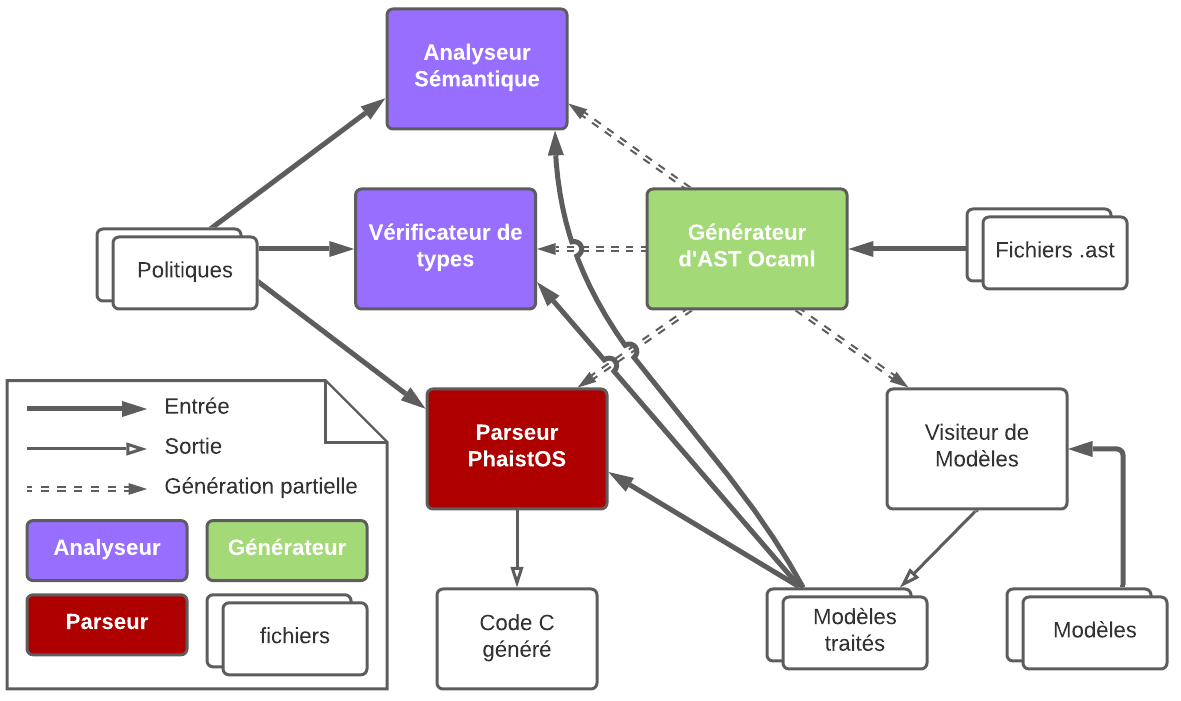
\includegraphics[width=\textwidth]{images/compiler}
    \caption{Schéma de fonctionnement du compilateur.}
    \label{fig:compiler}
\end{figure}

\subsubsubsection{Les fichiers AST}
\label{ast_files}

On remarque sur ce schéma que certaines entités importantes, comme le parseur, 
sont issues d'une génération partielle, cela signifie que certains des fichiers 
du code source utilisés par le parseur sont générés. Le générateur en question 
s'appelle ``le parseur d'arbre à syntaxe abstraite interrogeable'' (``Queryable 
AST Parser'' en anglais). Son but est de transformer une description d'AST (un 
arbre abstrait) contenue dans un fichier, en code source Ocaml pouvant 
modéliser chaque noeud de l'arbre (grace à un système d'objet propre au 
langage) et les parcourir à l'aide d'un visiteur dédié à cet arbre. Le fichier 
contenant ce code source généré s'appelle de manière générale \texttt{ast.ml}.

Par exemple, dans le cas du parseur, on fournira au générateur la description 
d'un AST qui définit la structure que doit avoir les politiques écrites par les 
utilisateurs. Cette description est contenue dans le fichier \texttt{phaistos.ast}
, dont un extrait est disponible sur la Figure~\ref{fig:policy_ast}. Comme 
on peut le voir dans l'extrait à la Ligne~\ref{script_rule}, on retrouve la 
racine de l'arbre appelée \texttt{script}, le point d'entré qui va contenir 
toutes les déclarations de haut niveau d'une politique PhaistOS dans la 
variable \texttt{topLevelStmts}. Comme préséntés dans la Partie~\ref{phlang}, 
on retrouve dans ces déclarations les définitions globales, l'état de la 
politique et la liste d'événements (Ligne~\ref{globdef}, Ligne~\ref{policydef} 
et Ligne~\ref{eventlist} respectivement).

\begin{figure}[h!t] \centering
    \begin{tabular}{c}
        \begin{lstlisting}[language=Phaistos-AST, linewidth=13.5cm]
script (topLevelStmts: topLevel list)(*\label{script_rule}*)
topLevel () >
    | globalDefinition (var: varDecl, initExpr: expression) (*\label{globdef}*)
    | policyDeclaration (vars: varDecl list)(*\label{policydef}*)
    ...
    | eventDeclaration (events: event list)(*\label{eventlist}*)
    ...
event (name: string, typeName: string option,
       vars: varDecl list)
...
        \end{lstlisting}
    \end{tabular}
    \caption{Extrait du fichier \texttt{phaistos.ast}.}
    \label{fig:policy_ast}
\end{figure}

Concrètement, le code Ocaml du générateur prend un fichier \texttt{.ast} en 
entrée et utilise les bibliothèques Menhir et Ocamllex pour parser son contenu. 
Il va ensuite générer une sortie sous forme de code source Ocaml qui contiendra 
une classe pour chaque noeud de l'AST (voir Figure~\ref{fig:equivalent_script})
. Le code contiendra aussi une classe d'objet \textbf{visiteur} avec une 
méthode \texttt{visit} pour chaque type de noeud, comme à la Ligne~\ref
{visitcall} où le noeud \texttt{script} accepte le visiteur en appellant la 
méthode \texttt{visit\_script}.

\begin{figure}[h!t] \centering
    \begin{tabular}{c}
        \begin{lstlisting}[language=Phaistos-AST, linewidth=15cm]
script (topLevelStmts: topLevel list) = 
  object(self)
    inherit astNode as super
    val mutable topLevelStmts = topLevelStmts
    // -- snip --
    method accept visitor = visitor#visit_script (self :> script)(*\label{visitcall}*)        
end
        \end{lstlisting}
    \end{tabular}
    \caption{Équivalent Ocaml du noeud \texttt{script}.}
    \label{fig:equivalent_script}
\end{figure}

\subsubsubsection{Le Visiteur de Modèles}
\label{templ_visitor}

Cette visite de noeud est importante car elle permettra au parseur par la suite 
de la parcourir la politique utilisateur et d'effectuer des actions 
particulières pour chaque noeud. Le comportement à adopter pour chaque noeud 
est décrit dans un \textbf{modèle}, et chaque modèle arbore un langage 
simplifié. Les modèles sont contenus dans des fichiers à part et nous 
permettent de maintenir le DSL facilement sans se préoccuper des lignes de code 
principales. Pour comprendre comment ils fonctionnent nous allons prendre 
l'exemple du modèle utilisé pour le noeud \texttt{event} (Figure~\ref
{fig:event_template}) qui va servir à générer le code C associé à un événement.

\begin{figure}[h!t]
    \centering
    \begin{lstlisting}[language=Phaistos-Template]
let! type =  [$ (*\label{type_decl}*)
  match my#typeName with | None -> "void" | Some x -> x $]    
let! signature = [" (*\label{sig_decl}*)
  static inline [$use "type"$] on_[$String.lowercase_ascii (*\label{type_call}*)
  my#name$] (struct iosched_data* dd[{if List.length
  my#vars > 0 then [","]}] [$forEach my#vars ",  "$])
"]
let! default = [{ (*\label{def_decl}*)
  ignore (self#atPut my#name (String (use "signature"))) }]
    \end{lstlisting}
    \caption{Le modèle \texttt{event}}
    \label{fig:event_template}
\end{figure}

Comme nous pouvons le voir aux Lignes~\ref{type_decl}~,~\ref{sig_decl}~et~\ref
{def_decl}, les modèles contiennent des régles dénotées par le mot clé \texttt
{!let}. Chaque règle est nommée et \texttt{default} est celle qui est 
interprétée en première, elle contient du code embarqué entre les délimiteurs 
\texttt{[\{} et \texttt{\}]} prévus à cet effet. Dans notre cas, le code Ocaml 
ici présent remplit une table de hachage maintenue par le visiteur actuellement 
sur le noeud \texttt{event} grâce à la méthode \texttt{atPut}, \texttt{self} 
étant le visiteur et \texttt{my} le noeud. La table de hachage associe au noeud 
de l'AST son équivalent textuel en C, pour cela elle appelle la règle \texttt
{signature} qui va produire une sortie textuelle (dénotée par les délimiteurs 
\texttt{["} et \texttt{"]}) de la signature de l'événement. Dans cette règle on 
peut insérer du code ayant pour but de générer une sortie sur place avec les 
délimiteurs \texttt{[\$} et \texttt{\$]} ou sans sortie particulière avec 
\texttt{[\{} et \texttt{\}]}. La règle \texttt{type} est appelée par \texttt
{signature} à la Ligne~\ref{type_call}, elle permettra d'écrire dans la 
signature le type de la fonction événement en cours de traitement.

Les modèles sont puissants, ils modularisent le comportement à adopter pour un 
noeud de l'arbre, tout en gardant un code relativement simple. On retrouve ce 
système de modèles dans d'autres parties du compilateur : \textbf{les 
analyseurs} (Partie~\ref{analyzers}) utilisent leur propres modèles pour 
exercer leurs vérifications statiques sur l'arbre.

Cependant, les modèles ne sont pas utilisables tels quels, le langage interne 
des modèles doit être interprété pour pouvoir être retranscrit en quelque chose 
de compilable par un langage. PhaistOS a donc dans son outillage un \textbf
{visiteur de modèles}, capable de parcourir ces derniers comme le fait le 
parseur pour les politiques utilisateur. Mais au lieu d'utiliser le fichier 
\texttt{phaistos.ast}, il utilisera le fichier \texttt{templateVisitor.ast}, 
qui décrit la structure des fichiers modèle. Le visiteur de modèles parcours 
donc ces derniers et les traite pour en ressortir un code Ocaml intégrable par 
le parseur ou les analyseurs. 

Concrètement, sur la Figure~\ref{fig:equivalent_script}, la méthode \texttt
{visit\_script} à la Ligne~\ref{visitcall} contiendra le contenu du modèle 
\texttt{script} traité par le visiteur de modèles.

\subsubsection{Vérification statique}
\label{analyzers}

Avant qu'une politique soit sujette à être compilée, il faut qu'elle soit 
validée par les différents analyseurs statiques de PhaistOS. En réalité, comme 
on le voit sur la Figure~\ref{fig:arch} en annexe, il existe trois analyseurs : 

\begin{enumerate}
    \item Un analyseur sémantique de base, contenu dans \texttt{Static-Analysis}
    , écrit en Ocaml. Il permettra de vérifier l'arborescence et la sémantique 
    de la politique de l'utilisateur final. Pour cela il vérifie des règles de 
    bases, comme le parenthésage ou la présence de certains champs obligatoires.
    \item Un analyseur de type contenu dans \texttt{TypeSystem}, écrit en OCaml 
    et qui vient compléter l'analyseur précédent. Il vérifiera que les types 
    utilisés dans la politique écrite par l'utilisateur sont corrects.
    \item Un vérificateur de propriétés de sécurité concernant l'utilisation de 
    l'API des requêtes d'E/S de Linux. Pour cela il utilise l'outil externe 
    Celf~\cite{schack2008celf} et est contenu dans \texttt
    {Linear-Logic-Analysis}.
\end{enumerate}

Mon stage n'a pas porté sur les analyseurs statiques, cependant les analyseurs 
écrits en Ocaml se rapprochent de par leurs fonctionnements, au reste du DSL 
(comme nous avons pu le voir dans la Partie~\ref{templ_visitor}), j'ai donc pu 
travailler certains de leurs aspects.

\subsubsection{PhaistOS dans Linux}

A mon arrivée sur le projet, PhaistOS utilisait un noyau Linux modifié, qui lui 
permettait d'inscrire ses propres politiques à la compilation du noyau à 
travers des fichiers de configuration. Le code source de la politique générée 
était intégré dans celui du noyau.

L'avantage d'une telle pratique est que le noyau utilisé reste le même et que 
les dépendances système de PhaistOS ne sont pas pertubées par les dernières 
mise à jour de Linux. L'inconvénient en revanche est que chaque nouvelle 
politique écrite par un utilisateur doit être intégrée au noyau, qui devra être 
recompilé par la suite.

\subsection{Et ensuite ?}

Dans toute cette architecture (Figure~\ref{fig:arch}, en annexe), PhaistOS fait 
preuve de forme et arrive a bien séparer les différentes tâches qui lui 
permettent d'arriver à sa finalité : générer un ordonnanceur d'E/S pour Linux.

Cependant, des aspects du compilateur restent à améliorer. Premièrement, la 
documentation du compilateur est très réduite, voir absente, que ce soit pour 
sa structure ou son API ; à mon arrivée sur le projet, PhaistOS était pour moi 
une énigme à résoudre. Étant donné que Nick n'était plus présent sur le projet, 
je n'avais que Nicolas Palix, mon tuteur, pour m'aider à assimiler les notions 
utilisée par le DSL (en faisant le parallèle avec le projet Ipanema~\cite
{lepers2020provable}). Il faudra donc apporter un effort de documentation pour 
le projet, y compris dans le code, dont l'absence de commentaires rend la tâche 
de compréhension encore plus ardue. --- ``\textit{Accompagné du mode de travail 
en distanciel et des tâches annexes, ce premier point m'aura prit un mois 
entier de mon stage.}''

Deuxièment, l'implémentation de PhaistOS dans le système n'est pas idéale car 
elle demande à l'utilisateur de recompiler tout son système pour qu'il puisse 
intégrer une nouvelle politique. L'objectif pour changer cela est de faire en 
sorte que les politiques générés par PhaistOS soient intégrable à chaud, dans 
le système.

Troisièmement, l'effort de compilation des différentes étapes de fonctionnement 
du DSL génèrent en somme une grande quantité d'avertissements, rendant 
illisible la sortie de la compilation Ocaml. Ce phénomène est principalement dû 
à la structure du code, qui fait de multiple inclusions d'un même fichier de 
fonctions, sans pour autant utiliser toutes les fonctions à chaque inclusion 
(plus de détails dans la Partie~\ref{warnings}). 

Pour finir, des détails concernant la structure ou l'implémentation du projet 
doivent être retravaillés, la plupart du temps ces aspects génants du 
compilateur sont le résultat d'une ancienne implémentation qui n'a pas été mise 
à jour par Nick :
\begin{enumerate}
    \item L'utilisation majeure de scripts shell dans les dossiers du DSL 
    empechait d'avoir une vision structurée de l'interaction que chacun pouvait 
    avoir avec les autres. Ce problème peut être réglé avec l'ajout de Makefile.
    \item Certains modèles présents dans PhaistOS sont erronés ou inutilisés.
    \item Les fichiers \texttt{.ast} contiennent d'anciennes règles 
    non-exploitées
    \item Les grammaires contenues dans les fichiers \texttt{.mly} utilisées 
    par la bibliothèque Menhir pour parser les politiques ou les modèles 
    contiennent des conflits qu'il faut corriger, sans quoi cela ajoute encore 
    plus de verbosité à la compilation du DSL.
\end{enumerate}

Dans l'ensemble, à mon arrivée, il y avait matière à travailler. L'état actuel 
de PhaistOS a fait que ma mission se prétait bien à sa description dans la 
Partie~\ref{mission}. Chacun des points cités précedemment à fait l'objet d'une 
de mes contributions durant le stage, dans le but d'améliorer le compilateur, 
et de le rendre plus accessible pour de nouveaux mainteneurs, qui comme moi 
doivent travailler sur le DSL.